\chapter{Dataset Collection}\label{chap:contrib1}


This contribution outlines the method used to collect a profiling dataset. The  dataset serves as a training set for the prediction model. The parameters covered are various Torchvision models and input sizes, execution time and power, both the inference and the training case as well as multiple GPUs and various GPU clocks.


\section{Operations}


In order to increase generality, our approach exploits the layer wise structure of DNNs by working at the layer level rather than the model level. In order to ensure rigor we must clarify our terminology. \\
On the layer level, the workload characteristics are determined by the layer and its input features. On this level, the objects with an identical characteristic workload are layers with specific settings and input feature dimensions. We will refer to these objects as operations. \\
At the model level, the objects with an identical characteristic workload are models with specific input dimensions. We will refer to these as model-input sets.\\ 
This study could have been conducted on the model level, the operations level or the kernel level.  \\
We chose the operations level over the kernel level, because it is  closer to the model level which determines the performance of real-world applications. We chose it over the model level itself, because all the combinations of operations open up a wider space of possibilities than the model level itself ever could. The operations level's relative proximity to the model level allows us to infer predictions for the model level behavior from it. \\
With these considerations, the units for which we will make predictions are individual operations. To this end, we collect a dataset of operations, profiling execution time and power for each individual operation. To ensure that the dataset reflects operations encountered in real-world scenarios, we selected a number of representative model-input sets from models of the Torchvision library. \\
Before profiling, the set of all operations occurring in any of these model-input sets is filtered using a manually defined whitelist of PyTorch layers. This whitelist excludes layers that contribute only negligible computational load, because their operations would introduce more measurement overhead than execution time data into the profiling results. Their inclusion would reduce the accuracy of the aggregation approach towards modeling full neural networks.

\section{Time Profiling}

\usetikzlibrary{shapes,arrows}
\usetikzlibrary{shapes.misc}
\usetikzlibrary{decorations.pathreplacing}

\begin{figure}[h!]
\centering

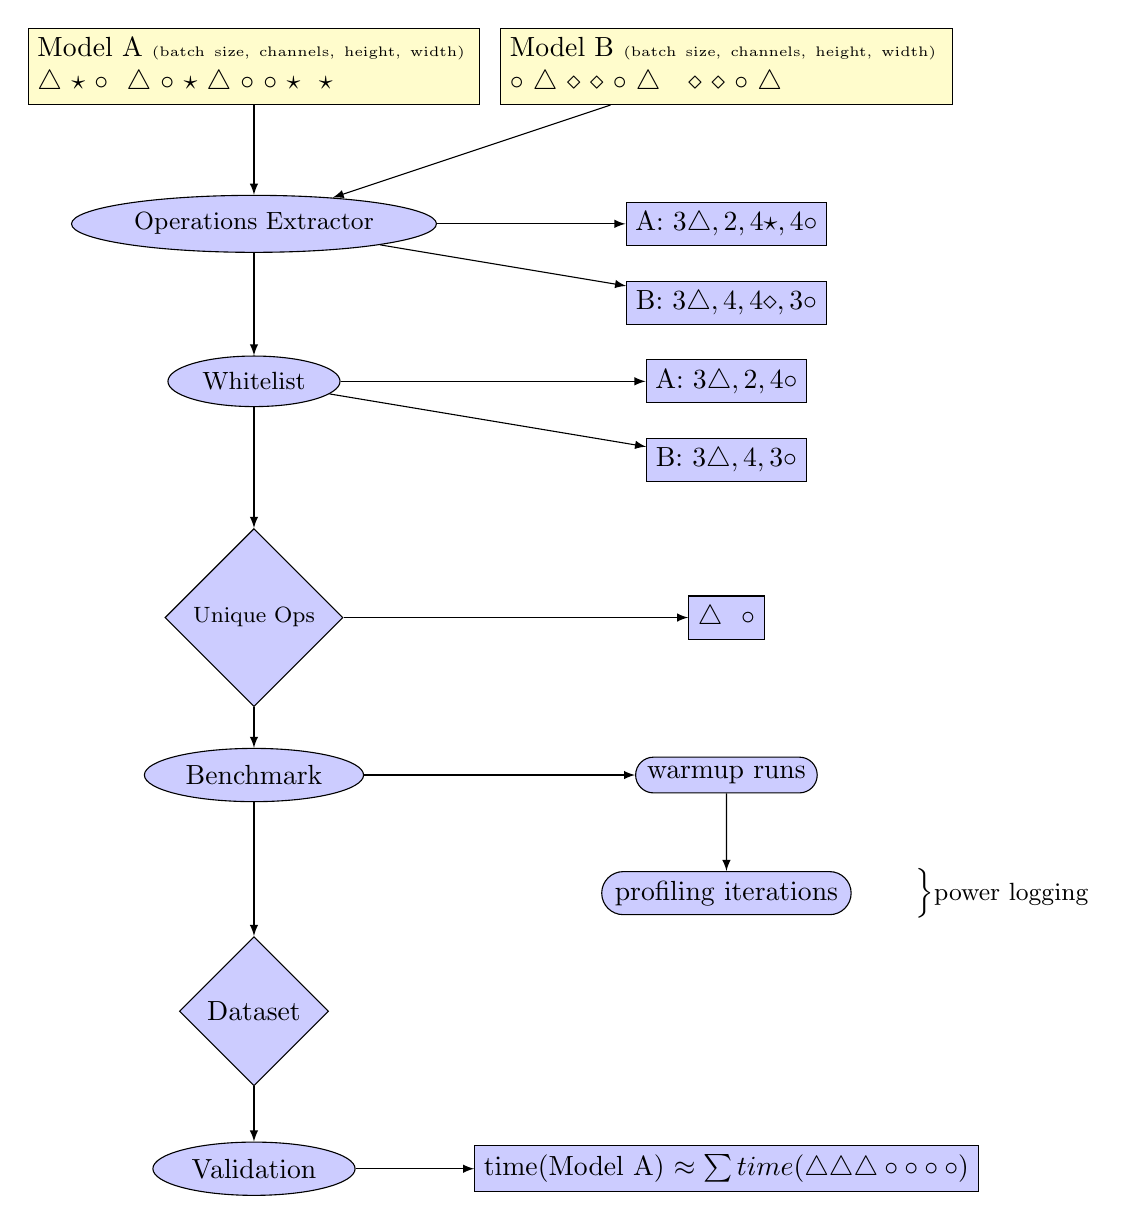
\begin{tikzpicture}[node distance=2cm]
    \node[rectangle, draw, fill=yellow!20, text width=5.5cm] (ellipse1) {Model A {\tiny(batch size, channels, height, width)}  $\triangle$ $\star$ $\circ$ $\square$ $\triangle$  $\circ$  $\star$ $\triangle$ $\circ$ $\circ$ $\star$  $\square$  $\star$};
  
  \node[rectangle, draw, fill=yellow!20, right of=ellipse1, node distance=6cm, text width=5.5cm] (ellipse2) {Model B {\tiny(batch size, channels, height, width)}  $\square$ $\circ$ $\triangle$  $\diamond$ $\diamond$ $\circ$ $\triangle$  $\square$ $\square$  $\diamond$ $\diamond$ $\circ$ $\triangle$  $\square$};

  \node[ellipse, draw, fill=blue!20] (opex) [below of=ellipse1, node distance=2cm] {\small Operations Extractor};

  \node[rectangle, draw, fill=blue!20] (stage2) [right of = opex, node distance=6cm] {A: $3\triangle, 2\square, 4\star, 4\circ$};

  \node[rectangle, draw, fill=blue!20] (stage1) [below of = stage2, node distance=1cm] {B: $3\triangle, 4\square, 4\diamond, 3\circ$};



  \node[ellipse, draw, fill=blue!20] (whitelist) [below of=opex, node distance=2cm] {\small Whitelist};

  \node[rectangle, draw, fill=blue!20] (stage3) [right of = whitelist, node distance=6cm] {A: $3\triangle, 2\square, 4\circ$};

  \node[rectangle, draw, fill=blue!20] (stage4) [below of = stage3, node distance=1cm] {B: $3\triangle, 4\square, 3\circ$};

  \node[diamond, draw, fill=blue!20] (unique) [below of=whitelist, node distance=3cm] {{\footnotesize Unique Ops}};

  \node[rectangle, draw, fill=blue!20] (benchset) [right of = unique, node distance=6cm] {$\triangle$ $\square$ $\circ$};

  \node[ellipse, draw, fill=blue!20] (bench) [below of=unique, node distance=2cm] {Benchmark};


  \node[rounded rectangle, draw, fill=blue!20] (proc1) [right of = bench, node distance=6cm] {warmup runs};

  \node[rounded rectangle, draw, fill=blue!20] (proc) [below of = proc1, node distance=1.5cm] {profiling iterations};
  
  % \draw[decorate,decoration={brace,mirror}] (proc.north east) -- (proc.south east) node[midway,xshift=3cm]{\small nvidia-smi power logging};

  \node[right of = proc, node distance = 3.5cm] {$\Big\}${\small power logging}};

  \node[diamond, draw, fill=blue!20] (dataset) [below of=bench, node distance=3cm] {Dataset};

  \node[ellipse, draw, fill=blue!20] (val) [below of=dataset, node distance=2cm] {Validation};

  \node[rectangle, draw, fill=blue!20] (sum) [right of = val, node distance=6cm] {time(Model A) $\approx \sum \text{time}(\triangle \triangle \triangle \circ \circ \circ \circ \square )$};

  % Define other nodes with shapes and text
%   \node[rectangle, draw, fill=blue!20] (start) [below of=ellipse1, node distance=3cm] {Start};
%   \node[diamond, draw, fill=red!20] (decision) [below of=start] {Decision};
%   \node[circle, draw, fill=green!20] (process) [right of=decision] {Process};
%   \node[rectangle, draw, fill=blue!20] (end) [below of=process] {End};

  % Draw arrows between nodes
  \draw[-latex] (ellipse1) -- (opex);
  \draw[-latex] (ellipse2) -- (opex);
  \draw[-latex] (opex) -- (stage1);
  \draw[-latex] (opex) -- (stage2);
  \draw[-latex] (opex) -- (whitelist);
  \draw[-latex] (whitelist) -- (stage3);
  \draw[-latex] (whitelist) -- (stage4);
  \draw[-latex] (whitelist) -- (unique);
  \draw[-latex] (unique) -- (benchset);
  \draw[-latex] (unique) -- (bench);
  \draw[-latex] (bench) -- (proc1);
  \draw[-latex] (proc1) -- (proc);
  \draw[-latex] (bench) -- (dataset);
  \draw[-latex] (dataset) -- (val);
  \draw[-latex] (val) -- (sum);



\end{tikzpicture}

\caption{Example models A and B illustrate the workflow. Operations within each model are represented as shapes. The Operations Extractor tracks each operation and its occurrence count in per model lists. The whitelist removes operations of negligible computational impact. From these lists, a global set of unique operations is created and then profiled in the Benchmark. Validation uses the per model lists to ensure aggregated times reflect full model execution.}
\label{fig:tikzexample}
\end{figure}

\vspace{1cm}

\input{Plots/runtime.tex}

The time profiling is performed using the benchmark utility from \texttt{torch.utils.benchmark} called Timer. This enables us to run our benchmark function with specific layers and input features as input parameters, allowing us to run it for individual operations. \\
To achieve more stable execution time profiling and improve the simultaneous power profiling we aggregate more statistics by running the benchmark for each operation for a duration of at least a few seconds. Different workload characteristics and different computational capabilities depending on the GPU configuration being profiled result in different requirements for individual profiling runs in order to ensure sufficient repetitions. In order to accommodate this requirement, the duration of the benchmark is configurable via a command-line parameters. \\
For the initialization of the operations instances within the benchmark script we have to be careful to avoid two extreme cases in order to achieve a sensible approximation of the execution characteristics within a neural network. The first case we want to avoid is initializing one instance of the operation and performing each benchmark loop on that instance. This would result in hitting the cash every time and would not be representative. The second extreme we want to avoid is initializing a new instance for each loop of the benchmark run, which would add the initialization overhead and the larger latency of having to access the GPU main memory every time, skewing our results in the opposite direction. We have therefore chosen the middle ground approach of initializing a sizable block of operation instances with random weights and biases, which are then looped over by the benchmark kernel, resulting in a moderate reuse of layers, stressing the memory system in a sensible manner. \\


\subsection{Inference}
The central difference between inference and training profiling appears in the design of the benchmark function. \\
For inference profiling we put our operations into \texttt{eval} mode and call them within a \texttt{torch.inference\_mode} environment, which is equivalent to the execution in a typical inference forward pass through a model. Within the loop we call the operator on a preinitialized random input tensor for the forward pass. The input tensor is a single instance, as it represents the activations from the previous layer which can be expected to live in high level memory in our memory hierarchy. Since this forward pass is everything we want to profile for inference, this benchmark loop is sufficient.

\subsection{Training}
For the training profiling we put our operations into \texttt{train} mode and omit the environment used in the inference case. In order to portray the training process for a single operation, we need to run a forward pass and a backward pass. The forward pass is still handled identically. In order to execute the backward pass we need a substitute for the gradients flowing backward trough the model. This is achieved by preinitializing a random torch vector with the dimensions of our operation's output which we can then call the backward pass on. Other than that, we only have to make sure the runtime retains the gradients for all operation instances for the appropriate duration and keep resetting the input vector gradients for each loop iteration.

\subsection{Proportionality}
Since our benchmark function assumes the number of benchmark iterations and the resulting total runtime to be proportional, we need to test that assumption. In order to do that, we plot their relationship in Figure \ref{fig:proport}. By identifying how short the total runtime needs to become for the linear relationship to break, we can find a lower bound to our desired benchmark duration for each operation we study. Our investigation reveals a lower bound of 100 ms. As every operation is benchmarked for at least several seconds in our actual measurements, we are well above that threshold and justified in assuming proportionality.


\section{Energy Profiling}

\input{Plots/startup.tex}

The energy profiling is conducted by measuring the power in watts. Combined with the time measurements this gives us the energy results. \\
We are starting \texttt{nvidia-smi} as a background process and logging the power readings into a temporary csv file, which is used to calculate each operation's power average. \\
A second instance of \texttt{nvidia-smi} runs during the complete benchmark process. The resulting log can be compared to the timestamps included in the dataset of profiled operations, in order to investigate surprising anomalies in the results. \\
Due to the nature of our measurement pipeline, some preparations and processing after the fact are necessary to ensure robust results. \\
As can be seen in Figure \ref{fig:startup1}, showing the power measurement over time for alternating idle times and benchmark calls, the transition is not instant. There are some power readings in between the steady states of idle and benchmark. \\
In order to illustrate the existence of a startup effect without idle times between the benchmark runs, Figure \ref{fig:startup2} shows five looped benchmark runs of the same benchmark overlayed. For each run we can observe the startup effect. \\
We do not want to keep this startup effect in our result, because it is a result of our benchmark execution and not representative of the much more integrated execution pipeline in a neural network.\\
In order to keep it from affecting our results, we use a $3\sigma$ channel around the initial mean of the power readings and drop everything outside the channel. \\
As a second precaution, the script also employs some warmup runs in order to further minimize the impact of the startup effect.\\


%However, the results relevant to our power profiling are calculated instantly from the temporary csv log file.

\section{Profiling Evaluation}


The following section explains the details of how we arrive at our results from log files collected in the benchmark runs. Below you can see a snippet from one of the log files. The third entry in each row is the power reading.

% \begin{small} % Change to \footnotesize or \scriptsize for even smaller text
\begin{verbatim}
2024/10/10 13:18:58.369, 81, 145.99, 4396, 11264
2024/10/10 13:18:58.407, 81, 182.11, 4396, 11264
2024/10/10 13:18:58.428, 81, 182.11, 4396, 11264
2024/10/10 13:18:58.439, 81, 182.11, 4396, 11264
2024/10/10 13:18:58.490, 81, 178.50, 4396, 11264
2024/10/10 13:18:58.514, 81, 178.50, 4396, 11264
2024/10/10 13:18:58.538, 81, 178.50, 4396, 11264
\end{verbatim}
% \end{small}

Let us begin with the power evaluation. The log file is read in via \texttt{pandas}\footnote{\href{https://pandas.pydata.org/}{pandas}}. Any existing rows containing a non-numerical value are dropped from the dataframe. We then find the standard deviation for the power and drop all rows containing a power reading outside a $3 \: \sigma $ range. The following formulae are used for the mean and standard deviation:

\begin{equation}
\overline{W} = \frac{1}{n} \sum_{i=1}^{n} W_i
\end{equation}

\begin{equation}
\sigma_W = \sqrt{\frac{1}{n - 1} \sum_{i=1}^{n} (W_i - \overline{W})^2}
\end{equation}

\begin{equation}
W_{filtered} = W \; \text{such that} \, |W - \overline{W}| < 3 \sigma_W
\end{equation}
    
With \( n \) being the number of timestamps and \( W \) being the power. \\
The same two formulae are used to find the mean power \( \overline{W}_{filtered} \) and standard deviation \( \sigma_{\overline{W}_{filtered}} \) of the filtered power. \\
Both the total runtime \(t_{tot}\) and its standard deviation \(\sigma_{t_{tot}} \) are provided by \texttt{torch.utils.benchmark}.\\
In the next step we find the total run energy \( E_{tot} \) and its error \( \sigma_{E_{tot}} \).

\begin{equation}
E_{tot} = \overline{W}_{filtered} \cdot t_{tot}
\end{equation}

\begin{equation}
\sigma_{E_{tot}} = \sigma_{\overline{W}_{filtered}} \cdot t_{tot}
\end{equation}

From this, we find the time per iteration \( t \) and the energy per iteration \( e \), as well as the error for the time per iteration \( \sigma_t \) and for the energy per iteration \( \sigma_e \) with the number of iterations being \( N \).

\begin{equation}
t = \frac{t_{tot}}{N}
\end{equation}

\begin{equation}
e = \frac{E_{tot}}{N}
\end{equation}

\begin{equation}
\sigma_t = \frac{\sigma_{t_{tot}}}{N}
\end{equation}

\begin{equation}
\sigma_e = \frac{\sigma_{E_{tot}}}{N}
\end{equation}

The most interesting results here are the time and energy per iteration with their respective errors, as well as the average power.

% 3 sigma cutoff
% warmup runs, also applying to time measurement of course

\section{GPU Clocks}
The last parameter we needed to build a test methodology for is the GPU core clock. A dedicated clocking script\footnote{Because using \texttt{nvidia-smi} to change the clock requires lower level permissions, this was done in a separate script with additional permissions, which was then called from the \texttt{sbatch} script used to run the benchmark.} takes command line parameters to set the desired clock speed. A range of clock speeds was tested in order to gain insight into the relationships between clock speed, runtime and energy consumption.

